\documentclass[UTF8, a4paper]{report}
\usepackage[margin=0.5in]{geometry}
\usepackage{graphicx}
\usepackage{xetexko}

\title{%
    <컴퓨터프로그래밍 3> 실습 보고서 \\ 
    \large [제 08 주] 리스트 성능측정 2}
\author{201704150 허강준}
\date{\today}


\begin{document}
    \maketitle
    \tableofcontents

    \chapter{프로그램 설명서}
        본 보고서에서는 정렬 리스트와 비정렬 리스트를 정의하고 여러 동작의 성능을 측정한 뒤 그 결과를 서로 비교해보는 프로그램에 대해 기술한다.

        \section{프로그램의 전체 설계 구조 (MVC 등)}
            
            \paragraph{%
                \normalfont 본 프로그램은 크게 프로그램의 제어를 담당하는 Controller인 \texttt{app\_controller}, 입/출력을 담당하는 View인 \texttt{app\_view}, 그리고 비정렬 리스트 모델 \texttt{unsorted\_list}와 정렬 리스트 모델인 \texttt{sorted\_list}, 성능 측정 타이머 모델인 \texttt{perf\_timer}, 그리고 테스트 파라메터 관리를 위한 \texttt{parameter\_set}등으로 나뉜다. 또한 리스트 처리를 위하여 C++의 Standard Template Library에 정의된 \texttt{vector} Type을 지난 과제에서 가져왔다.
            }
            
        \section{함수 설명서}
            
            \paragraph{\texttt{VECTOR(type)}}
            \paragraph{%
                \normalfont C++의 Standard Template Library에 정의된 Container Template Type인 \texttt{vector}를 일부 구현하였다. 구현된 메서드는 \texttt{new},  \texttt{delete}, \texttt{at}, \texttt{front}, \texttt{back}, \texttt{data}, \texttt{empty}, \texttt{size}, \texttt{max\_size}, \texttt{clear}, \texttt{insert}, \texttt{erase}, \texttt{push\_back}, \texttt{pop\_back}, \texttt{swap} 이다.
            }

            \paragraph{\texttt{parameter\_set\_new}}
            \paragraph{%
                \normalfont 파라메터 세트 생성자
            }

            \paragraph{\texttt{parameter\_set\_new\_with}}
            \paragraph{%
                \normalfont 최소 테스트 케이스 수, 최대, 증가 수를 인자로 받는 parameter\_set 생성자
            }

            \paragraph{\texttt{parameter\_set\_delete}}
            \paragraph{%
                \normalfont 파라메터 세트 소멸자
            }

            \paragraph{\texttt{parameter\_set\_set\_min\_test\_size}}
            \paragraph{%
                \normalfont 최소 테스트 케이스 수를 설정
            }

            \paragraph{\texttt{parameter\_set\_get\_min\_test\_size}}
            \paragraph{%
                \normalfont 최소 테스트 케이스 수를 반환
            }

            \paragraph{\texttt{parameter\_set\_set\_interval\_size}}
            \paragraph{%
                \normalfont 테스트 케이스 증가 수를 설정
            }

            \paragraph{\texttt{parameter\_set\_get\_interval\_size}}
            \paragraph{%
                \normalfont 테스트 케이스 증가 수를 반환
            }

            \paragraph{\texttt{parameter\_set\_set\_number\_of\_tests\_size}}
            \paragraph{%
                \normalfont 총 테스트 수 설정
            }

            \paragraph{\texttt{parameter\_set\_get\_number\_of\_tests\_size}}
            \paragraph{%
                \normalfont 총 테스트 수를 반환
            }

            \paragraph{\texttt{parameter\_set\_max\_test\_size}}
            \paragraph{%
                \normalfont 입력된 최소 테스트 케이스 수 및 증가 수, 총 테스트 수를 이용하여 최대 테스트 케이스 수를 반환
            }

            \paragraph{\texttt{perf\_timer\_new}}
            \paragraph{%
                \normalfont 타이머 생성자
            }

            \paragraph{\texttt{perf\_timer\_delete}}
            \paragraph{%
                \normalfont 타이머 소멸자
            }

            \paragraph{\texttt{perf\_timer\_start}}
            \paragraph{%
                \normalfont 타이머 시작
            }

            \paragraph{\texttt{perf\_timer\_stop}}
            \paragraph{%
                \normalfont 타이머 종료
            }

            \paragraph{\texttt{perf\_timer\_duration}}
            \paragraph{%
                \normalfont 측정된 시간 반환
            }

            \paragraph{\texttt{appview\_out}}
            \paragraph{%
                \normalfont 문자열 출력 및 개행
            }

            \paragraph{\texttt{app\_controller\_init\_performance\_measurement}}
            \paragraph{%
                \normalfont \texttt{parameter\_set}에서 관리할 최소 테스트 케이스 수, 증가 수, 총 테스트 수를 초기화
            }

            \paragraph{\texttt{app\_controller\_create}}
            \paragraph{%
                \normalfont 컨트롤러 생성자
            }

            \paragraph{\texttt{app\_controller\_time\_for\_unsorted\_array\_list\_remove\_max}}
            \paragraph{%
                \normalfont 최대값 삭제 테스트를 수행하고 수행 시간을 반환
            }
            
            \paragraph{\texttt{app\_controller\_time\_for\_unsorted\_array\_list\_add}}
            \paragraph{%
                \normalfont 리스트 추가 테스트를 수행하고 수행 시간을 반환
            }
            
            \paragraph{\texttt{app\_controller\_generate\_test\_data\_by\_random\_numbers}}
            \paragraph{%
                \normalfont 현재 시간을 기반으로 한 유사랜덤 테스트 데이터를 생성
            }
            
            \paragraph{\texttt{app\_controller\_show\_results}}
            \paragraph{%
                \normalfont 측정 결과를 출력
            }
            
            \paragraph{\texttt{app\_controller\_run}}
            \paragraph{%
                \normalfont 프로그램 메인 루틴 정의
            }
            
            \paragraph{\texttt{app\_controller\_delete}}
            \paragraph{%
                \normalfont 컨트롤러 소멸자
            }

            \paragraph{\texttt{unsorted\_array\_list\_is\_empty}}
            \paragraph{%
                \normalfont 비정렬 리스트가 비었는지 검사
            }

            \paragraph{\texttt{unsorted\_array\_list\_is\_full}}
            \paragraph{%
                \normalfont 비정렬 리스트가 꽉 찼는지 검사
            }

            \paragraph{\texttt{unsorted\_array\_list\_add}}
            \paragraph{%
                \normalfont 비정렬 리스트에 요소를 추가
            }

            \paragraph{\texttt{unsorted\_array\_list\_min\_position\_recursively}}
            \paragraph{%
                \normalfont 비정렬 리스트의 최솟값의 인덱스를 재귀적으로 탐색하고 리턴
            }

            \paragraph{\texttt{unsorted\_array\_list\_min}}
            \paragraph{%
                \normalfont 비정렬 리스트의 최솟값을 탐색
            }

            \paragraph{\texttt{unsorted\_array\_list\_remove\_max}}
            \paragraph{%
                \normalfont 비정렬 리스트의 최댓값을 리스트에서 제거
            }

            \paragraph{\texttt{unsorted\_array\_list\_max\_position\_recursively}}
            \paragraph{%
                \normalfont 비정렬 리스트의 최댓값의 인덱스를 재귀적으로 탐색하고 리턴
            }

            \paragraph{\texttt{sorted\_array\_list\_new}}
            \paragraph{%
                \normalfont 정렬 리스트 생성자
            }

            \paragraph{\texttt{sorted\_array\_list\_delete}}
            \paragraph{%
                \normalfont 정렬 리스트 소멸자
            }

            \paragraph{\texttt{sorted\_array\_list\_is\_empty}}
            \paragraph{%
                \normalfont 정렬 리스트가 비었는지 검사
            }

            \paragraph{\texttt{sorted\_array\_list\_is\_full}}
            \paragraph{%
                \normalfont 정렬 리스트가 꽉 찼는지 검사
            }

            \paragraph{\texttt{sorted\_array\_list\_position\_using\_binary\_search}}
            \paragraph{%
                \normalfont 정렬 리스트에 요소를 추가할 위치를 이진탐색 알고리즘을 이용하여 탐색
            }

            \paragraph{\texttt{sorted\_array\_list\_add}}
            \paragraph{%
                \normalfont 정렬 리스트에 요소를 추가
            }

            \paragraph{\texttt{sorted\_array\_list\_max\_position\_recursively}}
            \paragraph{%
                \normalfont 정렬 리스트의 최댓값의 위치를 재귀적으로 탐색
            }

            \paragraph{\texttt{sorted\_array\_list\_remove\_max}}
            \paragraph{%
                \normalfont 정렬 리스트의 최댓값을 리스트에서 제거
            }

            \paragraph{\texttt{sorted\_array\_list\_min\_position\_recursively}}
            \paragraph{%
                \normalfont 정렬 리스트의 최솟값의 위치를 재귀적으로 탐색
            }

            \paragraph{\texttt{sorted\_array\_list\_min}}
            \paragraph{%
                \normalfont 정렬 리스트의 최솟값을 탐색
            }

        \section{종합 설명서}

            \paragraph{%
                \normalfont 이번 프로그램은 8-1을 개선하여, 정렬 리스트의 여러 동작(최댓값 제거, 삽입, 최소값 탐색)을 정의하고 비정렬 리스트와의 성능 차이를 비교해볼 수 있도록 한다. 마찬가지로 \texttt{Vector} 타입을 이용하여 비정렬 및 정렬 리스트를 구현하고, 해당 리스트들에 대하여 테스트 케이스 별로 각각 삽입, 최솟값 탐색 및 최댓값 삭제 시간을 측정한다. 
            }
            
    \chapter{프로그램 장단점/특이점 분석}
            \section{비정렬 리스트 vs 정렬 리스트}
            \paragraph{%
                \normalfont 8-1에서 구현한 비정렬 리스트와는 다르게, 정렬 리스트에서는 원소간의 대소관계를 보장한다. 즉, 현재 원소는 이전 원소보다 크고 다음 원소보다 작으며, 항상 리스트의 끝에는 최대값이 위치한다는 의미이다. 따라서 삽입에 있어서는 O(n) 복잡도를 가지지만, 최소값 탐색이나 최댓값 삭제에 있어서는 O(1) 복잡도를 가진다.
            }   

            \section{자체 구현한 VECTOR(type)의 결함}
            \paragraph{%
                \normalfont 이전까지 사용된 \texttt{VECTOR(type)}의 경우 비정렬 리스트에서는 별 다른 문제가 발생하지 않았으나, 정렬 리스트에서 VECTOR(type)의 메서드 중 하나인 \texttt{VECTOR\_INSERT}를 실행하였을 때 Segmentation Fault가 발생하는 것을 확인하였다. 해당 함수를 디버깅 한 결과, 벡터에 삽입된 요소의 수가 삽입될 위치보다 클 경우 배열 내에서 요소들을 이동시키는 알고리즘에 문제가 있음을 확인하였는데, 반복 알고리즘을 진행할 때  \texttt{size} 에서 \texttt{pos}로 감소하는 것이 아닌 계속 증가하여 허가되지 않은 메모리를 참조하고 있었다. 따라서 반복자가 감소하도록 변경하였다. 또한 벡터를 생성하는 과정에서 사용한 \texttt{malloc}이 쓰레기 값을 제대로 제거하지 않아 삽입 과정에서 삽입 위치가 제대로 설정되지 않는 문제가 있었는데, 이는 \texttt{calloc}으로 수정하였다. 
            }

    \chapter{실행 결과 분석}
        \section{실행 결과 캡쳐}
        \begin{figure}[!htb]
            \centering
            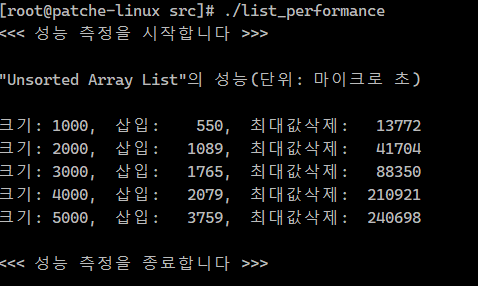
\includegraphics[width=\textwidth]{result.PNG}
            \caption{실행 결과1}
        \end{figure}
        
        \newpage

        \section{입력과 출력}
            실습 자료에서 제시된 테스트 데이터 생성 방법을 이용하였으며 출력 결과는 상기한 것과 같았음.
        \section{결과 분석}
            모든 입력에 대하여 정상적인 출력을 확인하였음.

    \chapter{소스코드}
        소스코드는 제출된 압축파일에 같이 동봉되어있으며 GitHub (0x00000FF/CNUCSE-Computer-Programming-III-2020-Spring) 에서도 열람할 수 있다.
\end{document}